There are many examples of Reference Architectures used in the commercial sector, but this section will focus on Reference Architectures that were clearly relevant to this effort. 

First, the \abbreviationFull[Small Unmanned Aircraft System]{SUAS} Reference Architecture developed at AFIT will be investigated. This is a relevant example as it fulfills the same general goals as the CubeSat Reference Architecture; namely, that it is for use in a design course series and is intended for students to use as a template for their design efforts. This SUAS Reference Architecture was started before this CubeSat effort and provides a useful baseline and inspiration, even if it is for a different domain. AFIT professors Dr. Jacques and Dr. Cox developed this architecture using Cameo Systems Modeler to describe a generic SUAS as described by the Army Research, Development, and Engineering Command, focused primarily on specific product output for the SUAS specialization track \citep{Jacques2019}. The SUAS Reference Architecture contains a Basic Ground Station Model, a Basic Multi-Rotor System Model, a Component Library, and sample build using the architecture.  The SUAS Reference Architecture is designed to allow students to easily build to a design specification from COTS components in the Component Library and test those designs using built-in parametric diagrams. These concepts will be applied to the CubeSat Reference Architecture as well, adapted for use in the spacecraft design course series. 
\begin{figure}[ht]
    \centering
    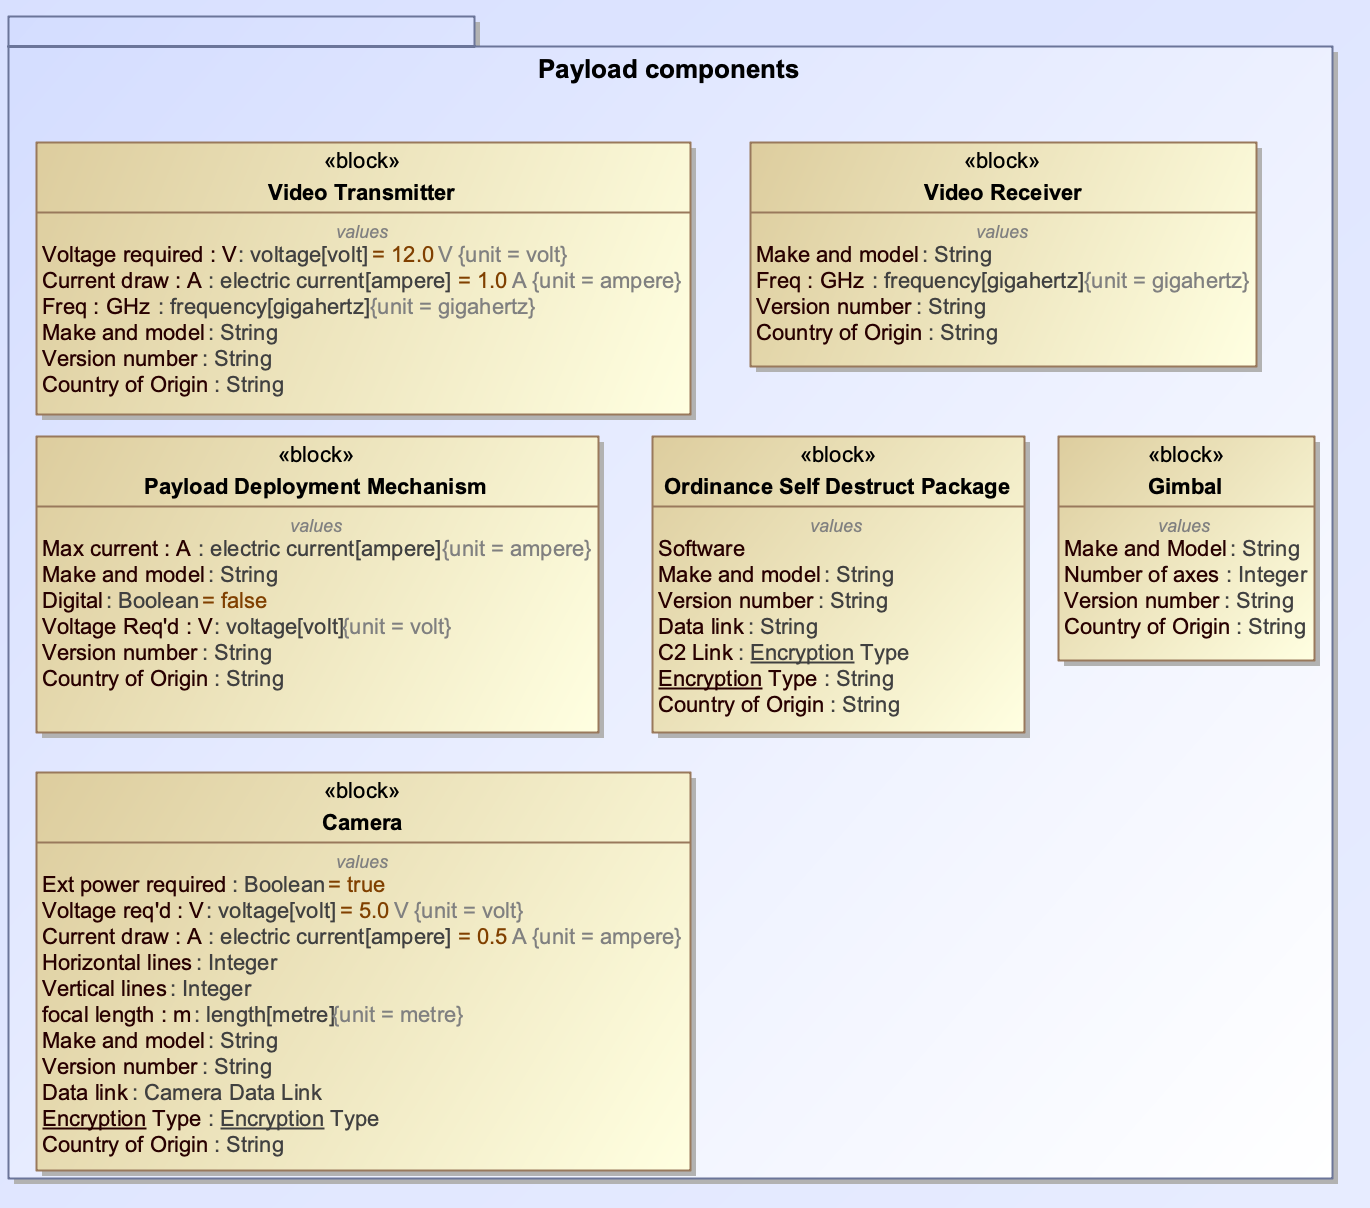
\includegraphics[width=\textwidth]{Thesis/Literature_Review/Lit Review Figures/suas component library.png}
    \caption{SUAS Component Library}
    \label{fig:SUAS Component Library}
\end{figure}



Jacques and Cox focused on the SUAS culture of rapid prototyping, and the Reference Architecture allows for designs to be developed at a much faster pace. The common template and vision provided through the model helps interdisciplinary teams design, build, and test SUAS systems with more time spent on producing a quality product, and less time spent designing the entire model from scratch \citep{Jacques2019}. Jacques and Cox captured their own extensive SUAS experience into their Reference Architecture, and the model will continue to be improved over time. Currently, it is being improved to streamline the cumbersome DoD Cybersecurity Risk Assessment process, using model elements to fill out required forms. The component library will also continually evolve as COTS components change. Figure \ref{fig:SUAS Component Library} shows a small section of their Component Library, providing blocks with value properties to start from. Figure \ref{fig:SUAS Organization} shows the SUAS Reference Architecture's top level organization, which this Reference Architecture will be modeled after for consistency. The component library, parametric diagrams, and general organization are useful in the development of the CubeSat Reference Architecture, but the spacecraft design course series has some unique differences that must be considered, such as instructor preferences and differing model scopes. 

\begin{figure}
    \centering
    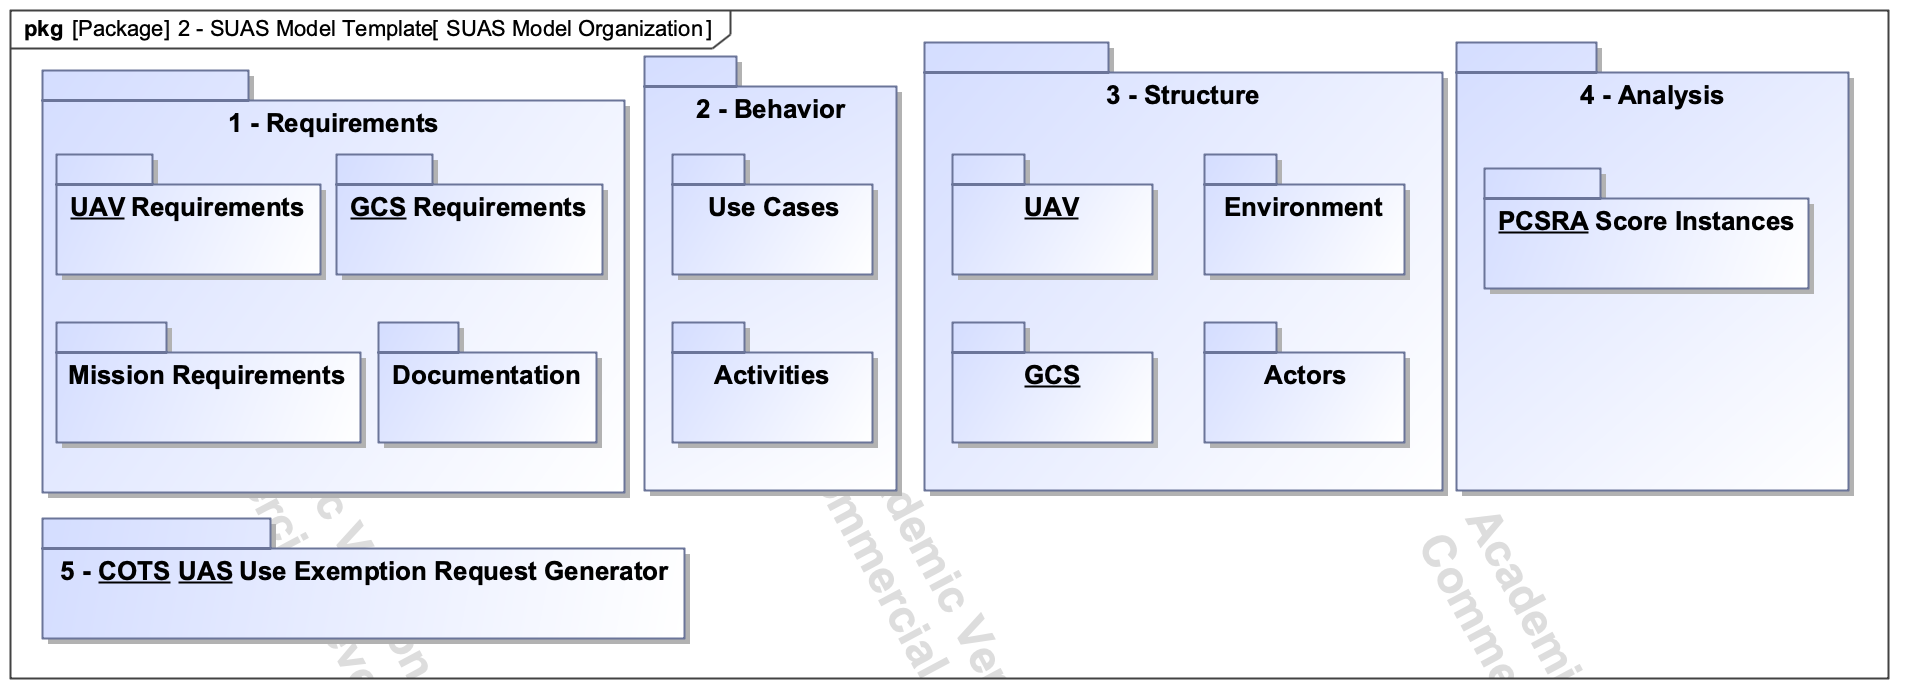
\includegraphics[width=\textwidth]{Thesis/Literature_Review/Lit Review Figures/suas organization.png}
    \caption{SUAS Organization}
    \label{fig:SUAS Organization}
\end{figure}

In the CubeSat domain, Kaslow and a group of Subject Matter Experts built a \abbreviationFull[CubeSat Reference Model]{CRM} as part of a partnership between the \abbreviationFull[Object Management Group]{OMG} and the \abbreviationFull[International Council on Systems Engineers]{INCOSE}. This CRM was intended to help CubeSat developers by providing logical, reusable architecture elements at a high level \citep{Kaslow2016}. Some sample diagrams are provided in their interim status updates \citep{CRM20,Kaslow2014,Kaslow2016,Kaslow2017,Kaslow2020,KaslowCRM3}, but the actual Cameo model was not available to investigate. This CRM describes three levels of architectural foundation that are necessary to capture the whole domain: the enterprise level, the space and ground segments, and the space and ground subsystems. Figure \ref{fig:CRM Domain} indicates the structure for the CubeSat domain as described by Kaslow et al.

\begin{figure}
    \centering
    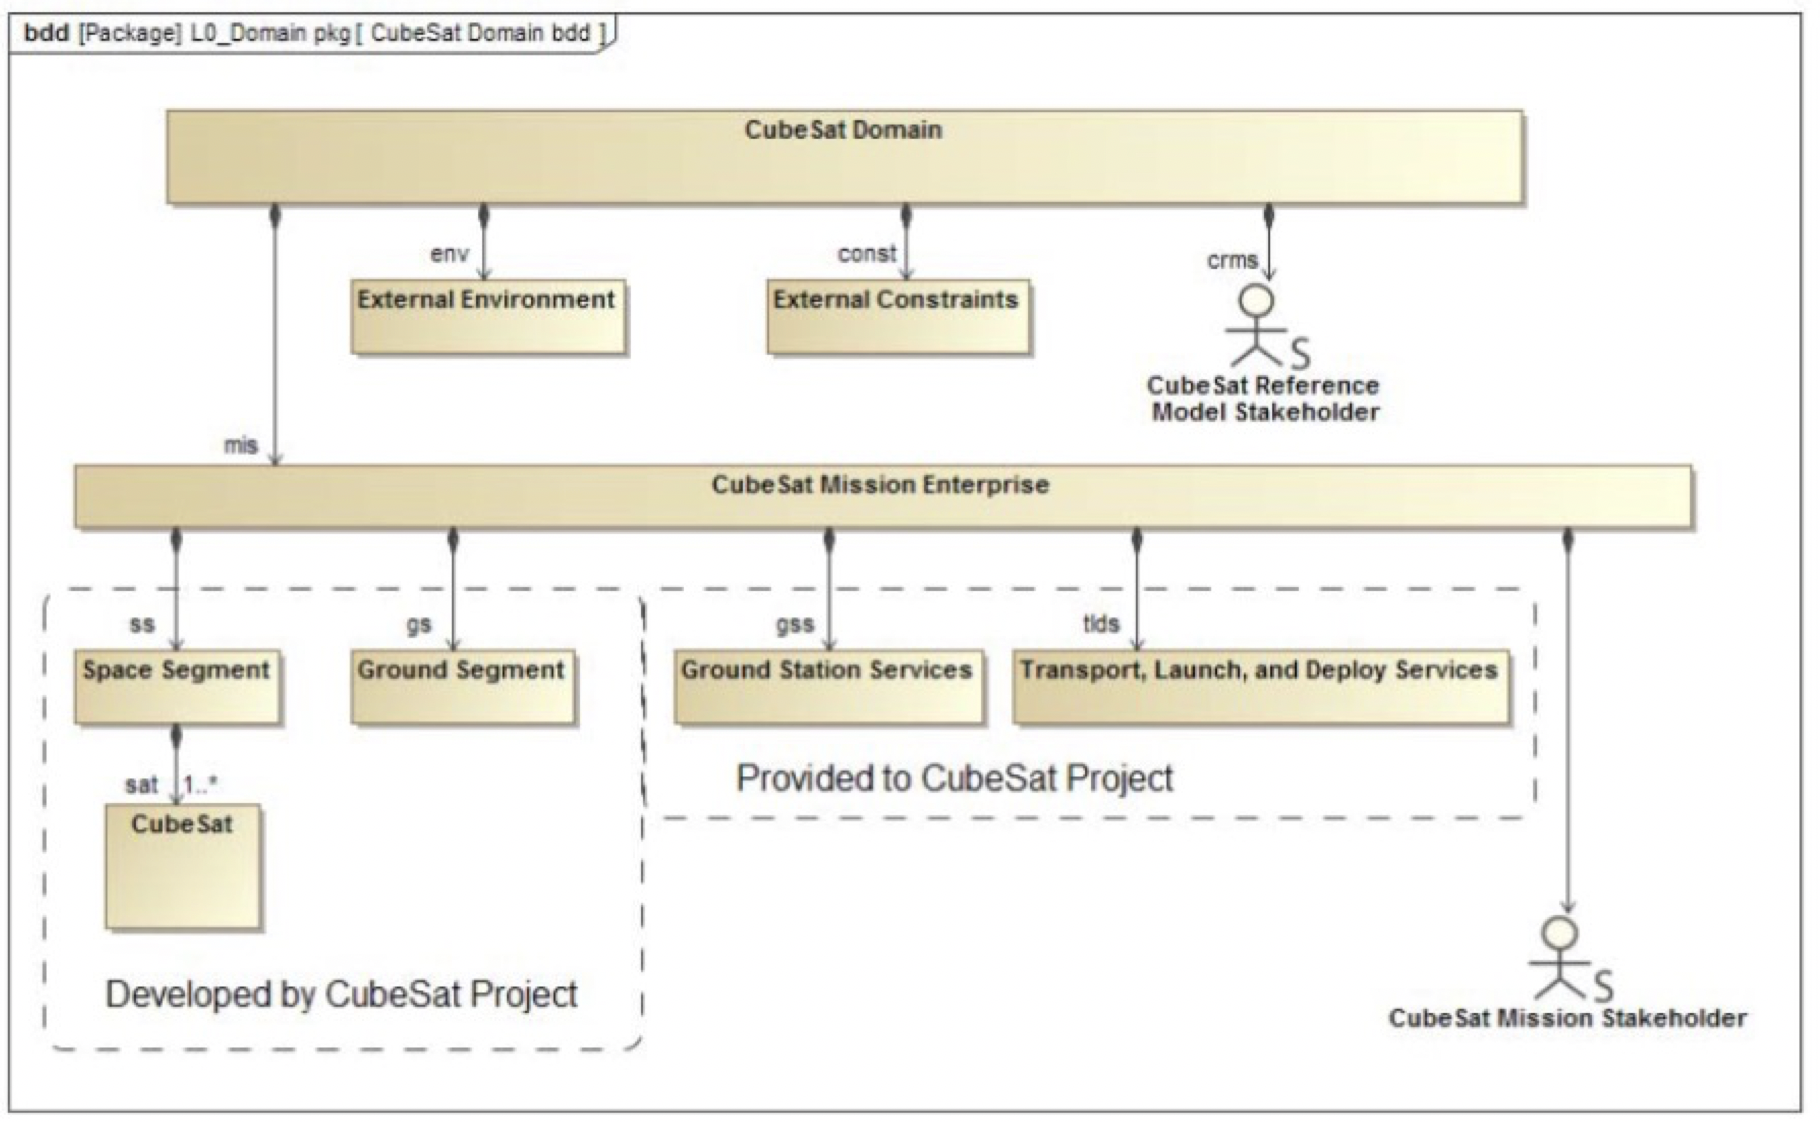
\includegraphics[width=\textwidth]{Thesis/Literature_Review/Lit Review Figures/CubeSat Domain.png}
    \caption{CRM CubeSat Domain}
    \label{fig:CRM Domain}
\end{figure}

Kaslow et al. used a block definition diagram to demonstrate the hierarchy of elements within the domain. They depict the CubeSat Mission Enterprise as being directly composed of a Space Segment, a Ground Segment, Ground Station Services, and Transport, Launch, and Deploy Services. Furthermore, they identified what must be developed by the CubeSat Project in greater detail, as shown by Figure \ref{fig:CRM RA Scope}.


\begin{figure}
    \centering
    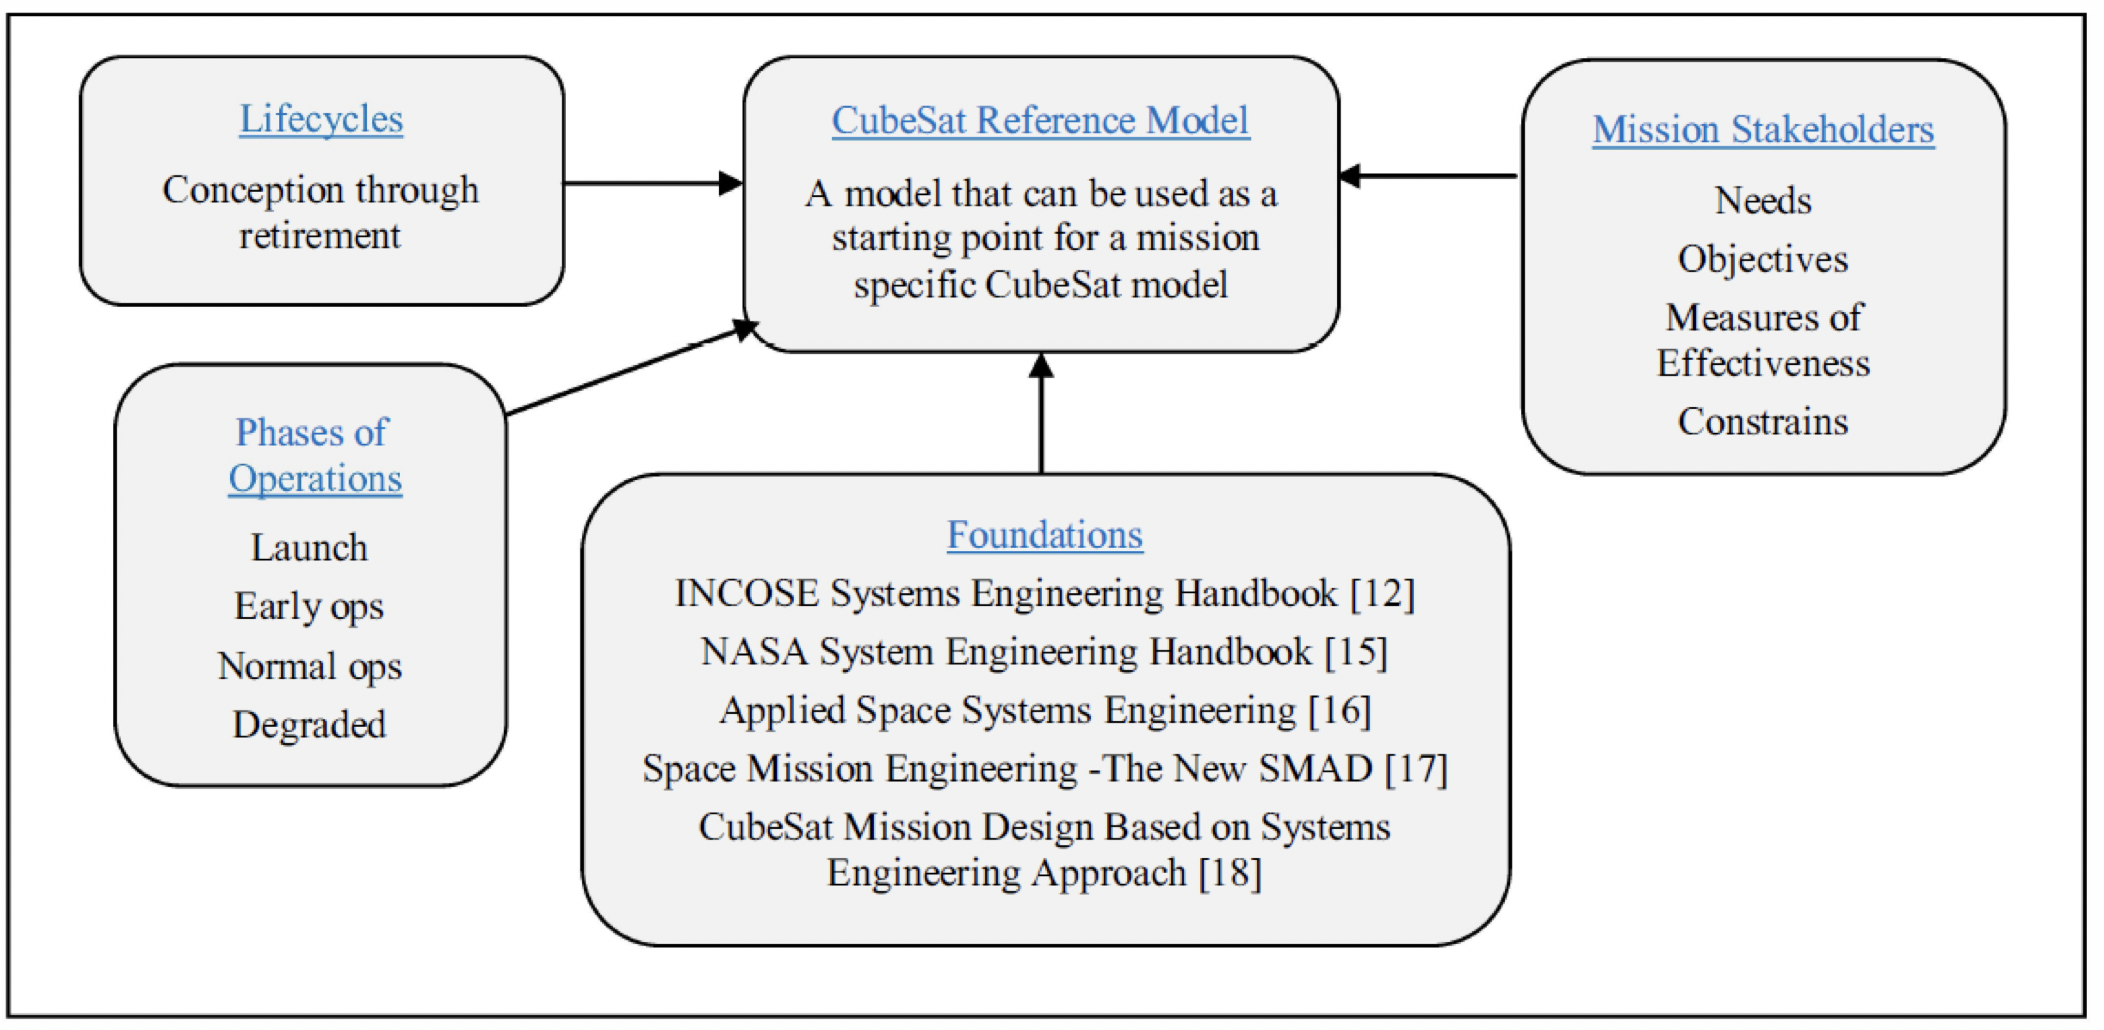
\includegraphics[width=\textwidth]{Thesis/Literature_Review/Lit Review Figures/CubeSat RA scope.png}
    \caption{CRM Scope}
    \label{fig:CRM RA Scope}
\end{figure}


\begin{figure}
    \centering
    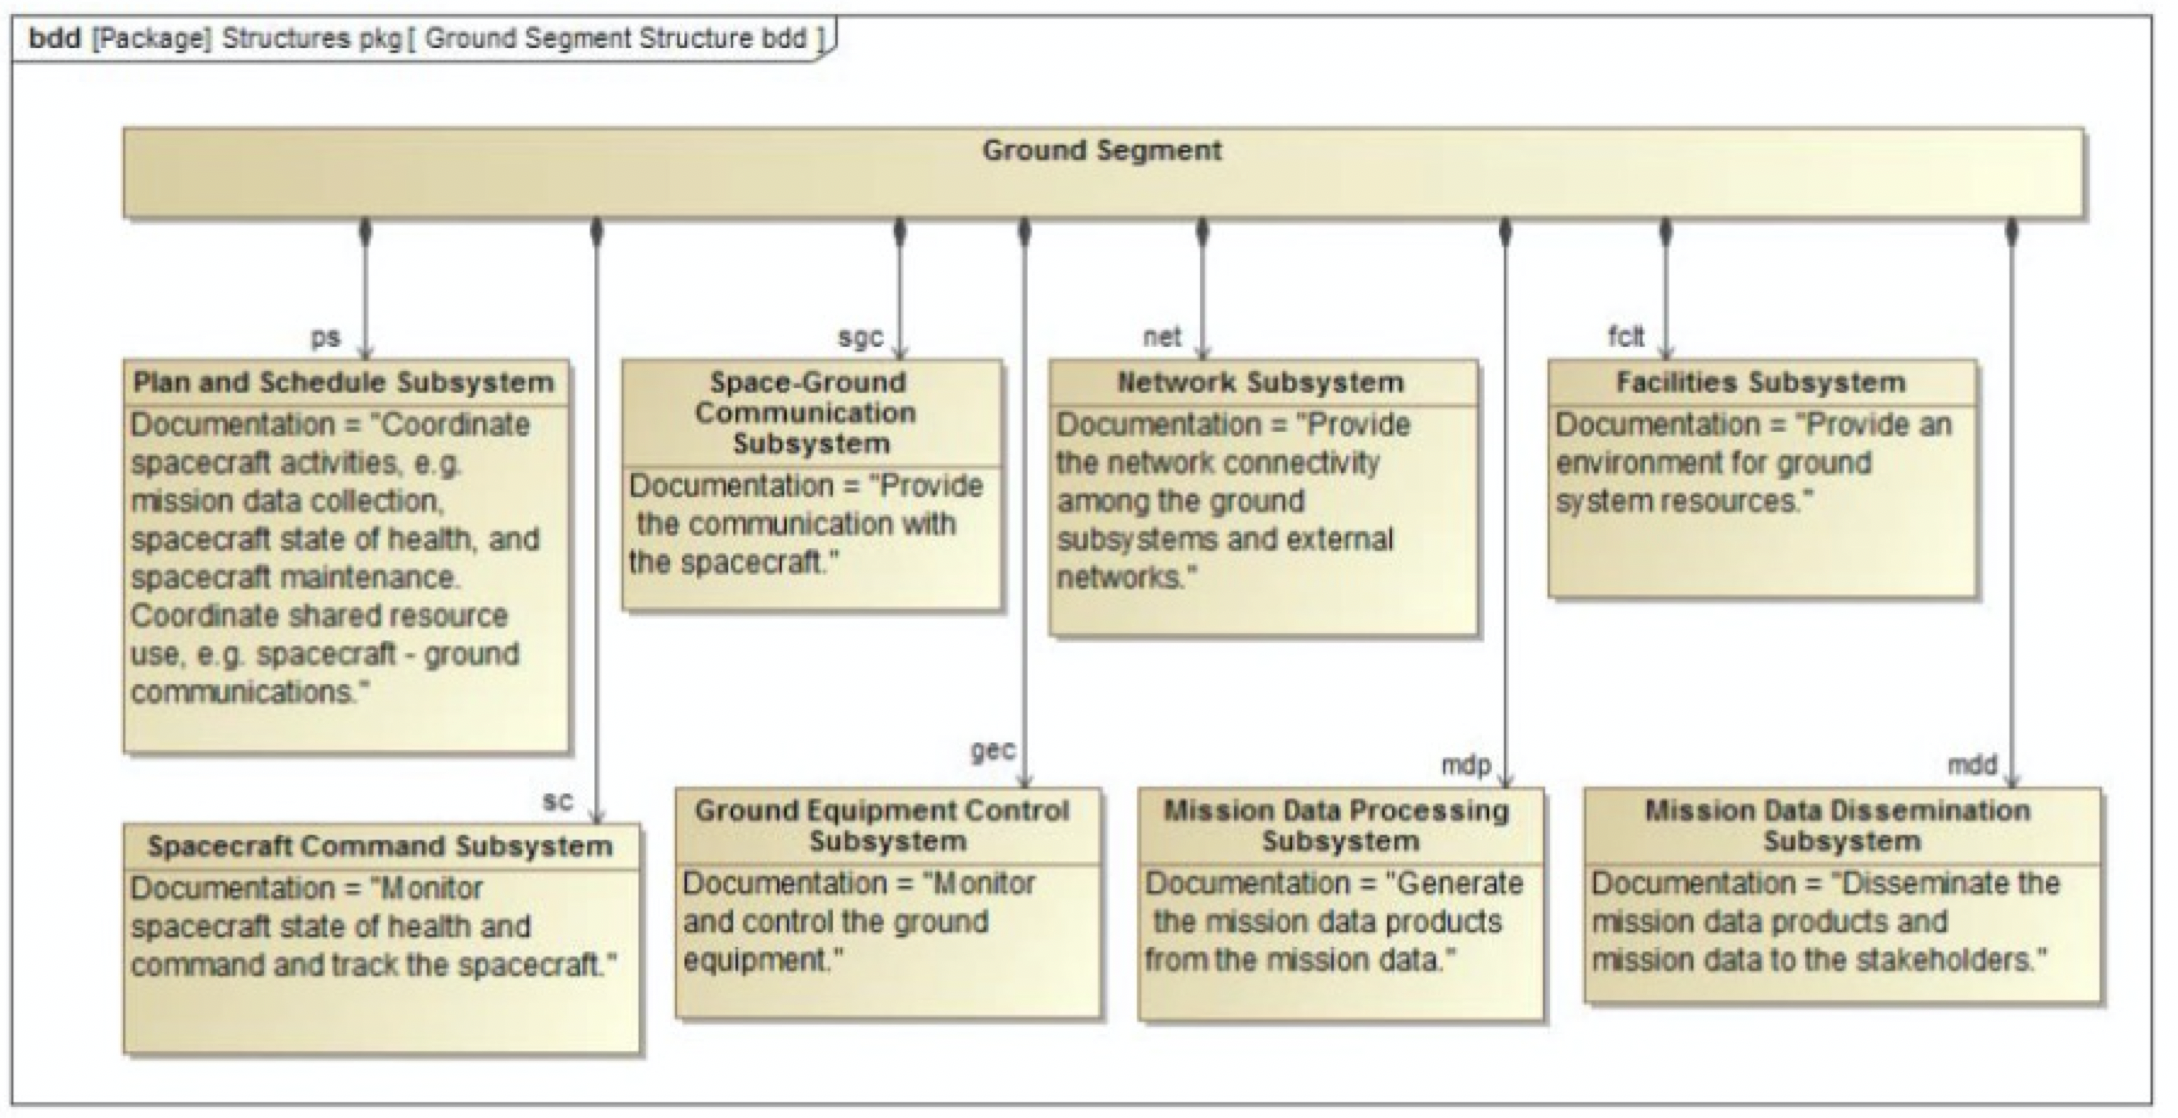
\includegraphics[width=\textwidth]{Thesis/Literature_Review/Lit Review Figures/CubeSat Ground Segment.png}
    \caption{CRM Ground Segment}
    \label{fig:CRM Ground Segment}
\end{figure}

\begin{figure}
    \centering
    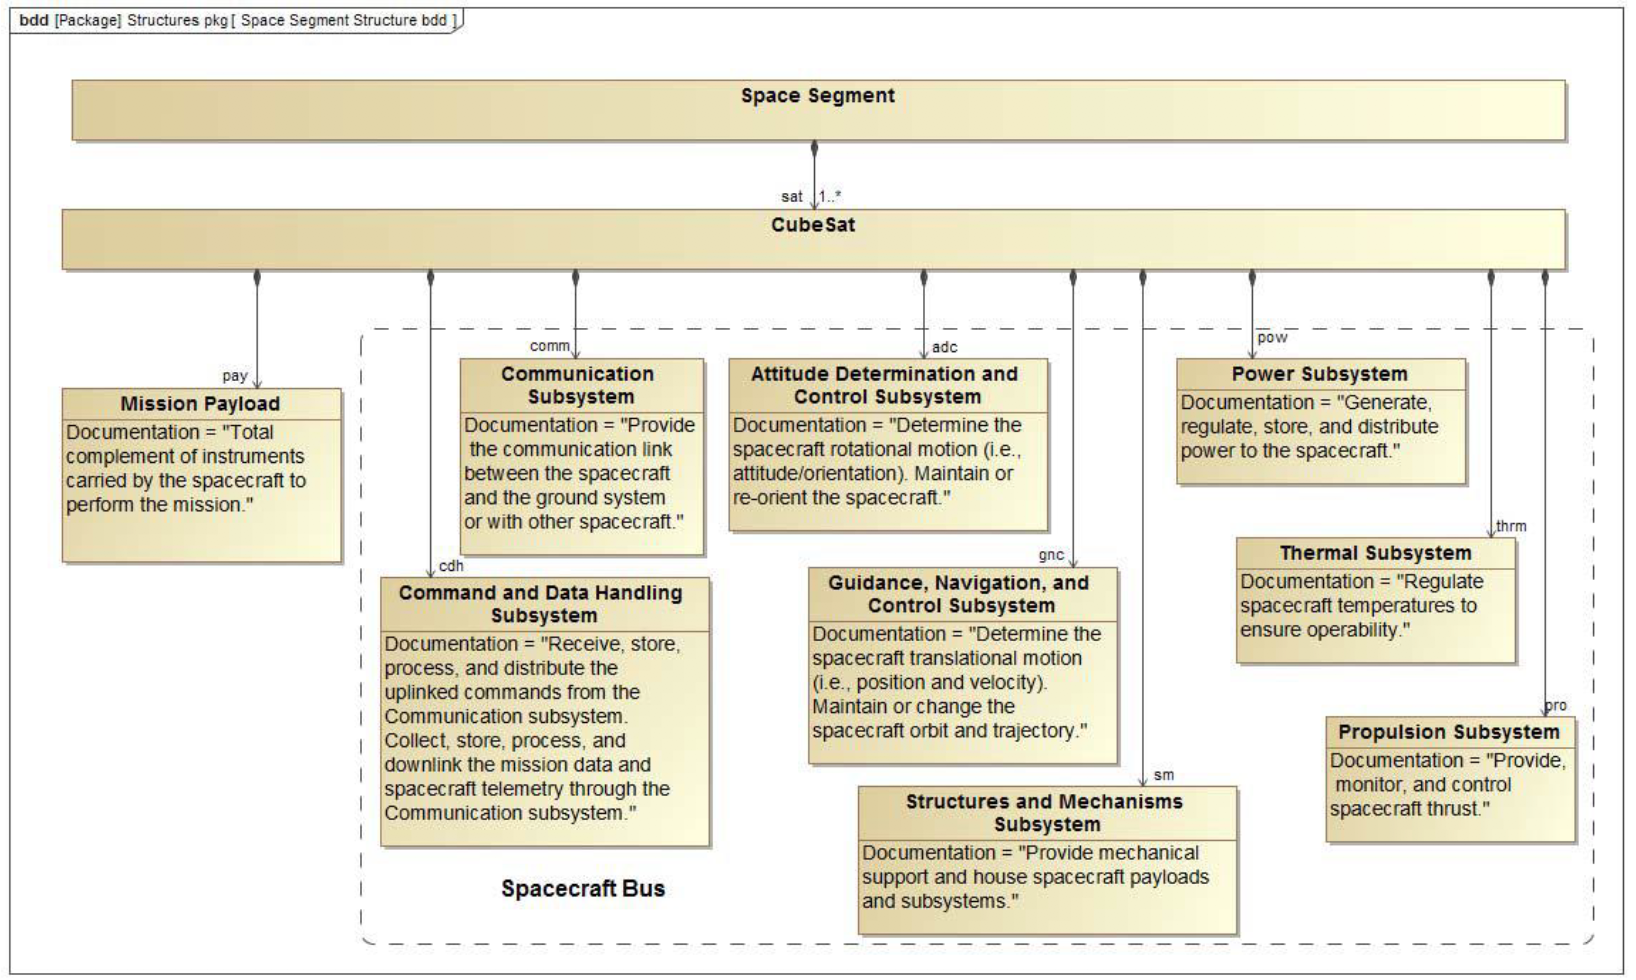
\includegraphics[width=\textwidth]{Thesis/Literature_Review/Lit Review Figures/CubeSat RA Space Segment.png}
    \caption{CRM Space Segment}
    \label{fig:CRM Space Segment}
\end{figure}


Kaslow et al. described all of the CubeSat subsystems and provided Block Definition Diagrams for the major views of a CubeSat, including each mission segment, as shown in Figure \ref{fig:CRM Ground Segment} for the Ground Segment and Figure \ref{fig:CRM Space Segment}.

Kaslow et al. determined that this logical architecture would provide guidance for CubeSat developers to begin to formulate their own mission specific architectures, knowing that their model did not have and could not have the specificity required to support every type of mission. It provided a top-level guide to how a CubeSat enterprise is organized, and some of the external stakeholders as well, as shown in Fig \ref{fig:CRM Stakeholders}. Their model is a starting point for mission specific teams to incorporate their unique knowledge to formulate their own reference architectures.

\begin{figure}
    \centering
    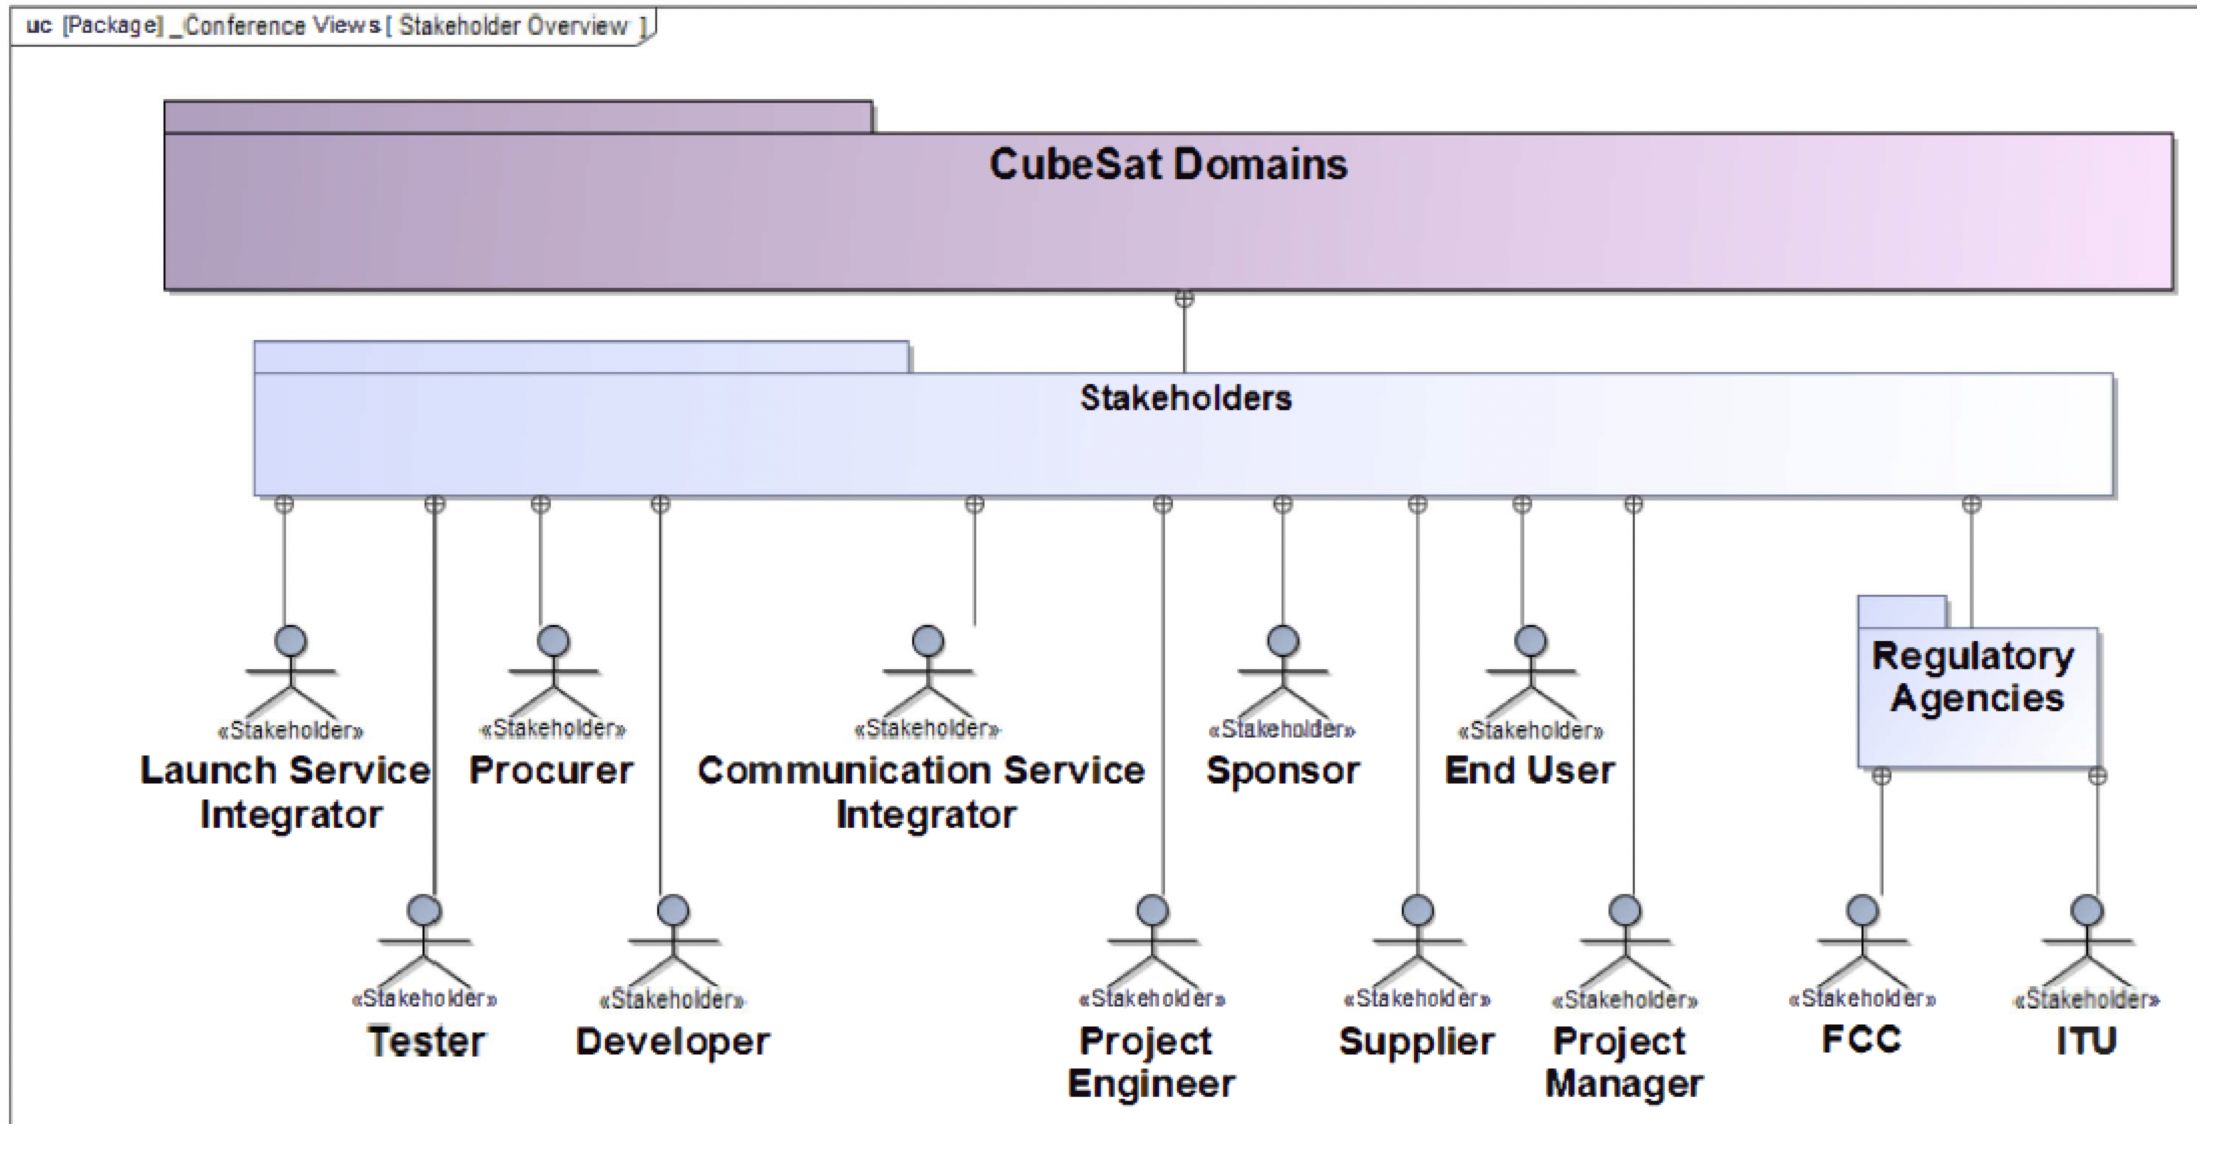
\includegraphics[width=\textwidth]{Thesis/Literature_Review/Lit Review Figures/CubeSat Stakeholders.png}
    \caption{CRM Stakeholders}
    \label{fig:CRM Stakeholders}
\end{figure}

After investigating the CRM status updates, however, the CubeSat Reference Model was missing much of the low-level details that was included in the SUAS Reference Architecture. A thorough reference architecture in this domain ought to include the high-level documentation and views of the CRM and the low-level component library and functionality of the SUAS reference architecture. 

Several other gaps exist that will be addressed in this thesis effort. First, the CRM is not designed for outputting traditional documents for system level reviews. There is no easy way to generate a \abbreviationFull[Concept of Operations]{CONOPS} document or \abbreviationFull[Operational Requirements Document]{ORD}, for example, and that is a desire for an AFIT CubeSat Reference Architecture. Second, the CRM does not appear to have a component library or a generic, intuitive system that can be easily adapted by students new to MBSE. Finally, the CRM does not appear to have sufficiently detailed value properties for the system to be useful for detailed mission analysis using MATLAB and STK. Students in the AFIT course series must design down to a very granular level of detail with many value properties for each subsystem in order to perform the required analysis and calculations. The CRM is quite useful though in examining what subject matter experts deem important for a CubeSat model and for their various subsystem internal block diagrams.

Another Reference Model that was investigated was the satellite model by Sanford Friedenthal \citep{FriedenthalArchitectingSpacecraft}. In his book, he walks through his version of a CubeSat model for the "FireSat II" mission, also using the OOSEM methodology and Cameo Systems Modeler. His book provides very helpful diagrams and best practices and will prove to be a key inspiration for this Reference Architecture. 

Should I even cite Luke Farrell's thesis? I didn't really use anything from his model...